\chapter{Isomorphic Theorems}

\section{Normal Subgroups}

\begin{definition}[Normal Subgroup]\index{normal subgroup}\label{def:normal-subgroup}
    Let $G$ be a group and $N$ be a subgroup. We say $N$ is a \term{normal subgroup} of $G$, denoted $N \triangleleft G$, if \[
        \forall g \in G, gN = Ng.
    \] Equivalently, if $gNg^{-1} = N$.
\end{definition}

\begin{definition}[Simple Group]\index{simple group}\label{def:simple-group}
    A group $G$ is \term{simple} if it has no nontrivial normal subgroups.
\end{definition}

\begin{example}
    Kernels of group homomorphisms are normal subgroups.

    \begin{proof}
        Let $x \in \ker{\phi}$ for some homomorphism $\phi: G \to H$.

        Then, $\phi(gxg^{-1}) = \phi(g)\phi(x)\phi(g)^{-1} = \phi(g)e\phi(g)^{-1} = e$.

        Therefore, $gxg^{-1} \in \ker{\phi}$.
    \end{proof}
\end{example}

It is important to note that some group are normal under one group but not under another.

\begin{example}
    The alternating group, $A_n$, is normal in the symmetric group, $S_n$.

    This is because $A_n$ is the kernel of the sign homomorphism, which is a normal subgroup by the previous example.

    {~~~}

    For example, consider $S_3$ and $A_3$. \[
        S_3 = \{e, (12), (13), (23), (123), (132)\}, \quad A_3 = \{e, (123), (132)\}.
    \]

    We have $(13)A_3(13) = \{
        (13)e(13), (13)(123)(13), (13)(132)(13)
        \} = \{
        e, (132), (123)
    \} = A_3$.
\end{example}

\section{Isomorphism Theorem}

\begin{definition}[Quotient Group]\index{quotient group}\label{def:quotient-group}
    Let $G$ be a group and $N$ a normal subgroup. Then, we can define the \term{quotient group} $G/N$ as the set of left cosets of $N$ in $G$ with the operation \[
        (gN)(hN) := (gh)N.
    \]
\end{definition}

% \begin{proof}
%     WTS $(gh)N$ is a group. 

%     \begin{enumerate}
%         \item \textbf{Closure:} Let $g_1N, g_2N \in G/N$. Then, \[
%             (g_1N)(g_2N) = (g_1g_2)N \in G/N.
%         \]
%         \item \textbf{Associativity:} Let $g_1N, g_2N, g_3N \in G/N$. Then, \[
%             (g_1N)((g_2N)(g_3N)) = (g_1N)(g_2g_3)N = (g_1g_2g_3)N = (g_1g_2)g_3N = ((g_1N)(g_2N))(g_3N).
%         \]
%         \item \textbf{Identity:} Let $eN \in G/N$. Then, \[
%             (gN)(eN) = (ge)N = gN = (eg)N = (eN)(gN).
%         \]
%         \item \textbf{Inverses:} Let $gN \in G/N$. Then, \[
%             (gN)(g^{-1}N) = (gg^{-1})N = eN = (g^{-1}g)N = (g^{-1}N)(gN).
%         \]
%     \end{enumerate}
% \end{proof}

\begin{theorem}
    $G/N$ is a group if and only if $N \triangleleft G$.
\end{theorem}

\begin{example}
    $A_n$ is normal in $S_n$, so $S_n/A_n$ is a group.

    $A_n$ has $2$ cosets: itself, and the set of all odd permutations. Therefore, $S_n/A_n \cong \Z_2$.

    \begin{center}
        \begin{tabular}{c|c|c}
                      & $A_n$     & $(12)A_n$ \\ \hline
            $A_n$     & $A_n$     & $(12)A_n$ \\ \hline
            $(12)A_n$ & $(12)A_n$ & $A_n$
        \end{tabular}
        $\quad \cong \quad$
        \begin{tabular}{c|c|c}
                & $0$ & $1$ \\ \hline
            $0$ & $0$ & $1$ \\ \hline
            $1$ & $1$ & $0$
        \end{tabular}
    \end{center}

    We have $S_n/A_n \cong \Z/2\Z = \{ 0, 1 \} = \{ -1, 1 \}$.

    Moreover, since $\sgn: S_n \to \{ -1, 1 \}$, we see $S_n/\ker{\sgn} \cong \im{\sgn}$.
\end{example}

\begin{theorem}[The First Isomorphism Theorem]\index{first isomorphism theorem}\label{thm:first-isomorphism}
    Let $G$ be a group, and $\phi: G \to H$ be an homomorphism. Then, \[
        G/\ker{\phi} \cong \im{\phi}.
    \] and the isomorphism is given by \[
        \begin{matrix}
            G/\ker{\phi} & \to     & \im{\phi} \\
            g\ker{\phi}  & \mapsto & \phi(g)
        \end{matrix}
    \]
\end{theorem}

\begin{theorem}[The Correspondence Theorem]\index{correspondence theorem}\label{thm:correspondence}
    Let $G$ be a group, and $N \triangleleft G$. Then, there is a correspondence between the set of subgroups of $G$ containing $N$ and the set of subgroups of $G/N$. \[
        \begin{matrix}
            \left\{ H \le G \mid N \subseteq H \subseteq G \right\} & \longleftrightarrow & \{ K \le G/N \} \\
            H                                                       & \longleftrightarrow & H/N
        \end{matrix}
    \]
\end{theorem}

\begin{figure}[ht!]
    \centering

    \includegraphics[width=0.67\linewidth]{figures/correspondence-theorem.png}
\end{figure}

The first isomorphism theorem tells us how to reduce the complexity of the group, and the correspondence theorem tells us that we do not loose any information when we do so.

\begin{proposition}
    Let $G$ be a group, and $H$ a subgroup. Then $H$ is normal in $G$ if any only if there exists some homomorphism $\phi: G \to K$ to some group $K$ such that $H = \ker{\phi}$.
\end{proposition}

\begin{remark}
    Sometimes, it is difficult to prove that a subgroup is normal directly. However, if we can find a homomorphism with the subgroup as its kernel, then we can conclude that the subgroup is normal.
\end{remark}

\begin{definition}[Index]\index{index (of a subgroup)}\label{def:index}
    Let $H$ be a subgroup of $G$. The cardinality of $G/H$ is called the \term{index} of $H$ in $G$, denoted $[G:H]$.
\end{definition}

Informally, the index of a subgroup is the number of cosets of the subgroup in the group.

\begin{theorem}
    Let $G$ be a group and $H \le G$ of index $2$. Then, $H$ is normal in $G$.
\end{theorem}

We will construct a homomorphism $\phi: G \to \Z_2$ with $H = \ker{\phi}$, and thus $H \triangleleft G$.

\begin{remark}
    We often construct the homomorphism by manifesting some property of the subgroup.
\end{remark}

\begin{proof}
    Since $[G:H] = 2$, we have $G = H \sqcup g_0H$ for some $g_0 \in G \setminus H$.

    Define a function \[ phi: G \to \{ 1, -1 \} \] by \[
        \phi(g) = \begin{cases}
            1  & g \in H    \\
            -1 & g \in g_0H
        \end{cases}
    \]

    We claim that $\phi$ is a homomorphism. That means to prove $\phi(gh) = \phi(g)\phi(h)$ for all $g, h \in G$.

    In words, this means
    \begin{listu}
        \item $g, h \in H$ implies $gh \in H$

        This follows from the fact that $H$ is a subgroup.

        \item $g, h \notin H$ implies $gh \in H$

        % TODO
        % If $g, h \notin H$, then $g = g_0t_1$ and $h = g_0t_2$ for some $t_1, t_2 \in H$.

        \item $g \in H$ and $h \notin H$ implies $gh \notin H$

        If $g \in H$ and $h \notin H$, then $g \in H$ and $h \in g_0 H$.

        This means $\exists t \in H$ s.t. $h = g_0t$.

        Suppose for contradiction that $gh = g g_0 t \in H$.

        Then, $g_0 = g^{-1} (gh) t^{-1} \in H$, which is a contradiction.
    \end{listu}

    We conclude that $\phi$ is indeed a homomorphism.

    By definition, \[
        \ker{\phi} = \{ g \in G \mid \phi(g) = 1 \} = \{ g \in G \mid g \in H \} = H.
    \]

    Therefore, $H$ is normal in $G$.
\end{proof}

\begin{example}
    These are some examples of normal subgroups we have seen before.

    \begin{listo}
        \item Let $D_n$ be the dihedral group generated by $R$ and $S$. 
        
        $| D_n | = 2n$. 
        
        $\{ 1, R, \dots, R^{n-1} \} \cong C_n$ is a subgroup of index $2$, $[D_n : C_n] = 2$.

        Thus, $\{ 1, R, \dots, R^{n-1} \} \triangleleft D_n$.

        \item Let $\mathcal{R}$ be the group generated by Rubik's cube of $2 \times 2 \times 1$. 
        
        $| \mathcal{R} | = 48$.

        $V_1, V_2, H_1, H_2$ is a subgroup that generates $S_4$, so $[ \mathcal{R} : S_4 ] = 2$.

        Thus, $S_4 \triangleleft \mathcal{R}$.
    \end{listo}
\end{example}

\begin{theorem}
    Let $p$ be a prime number, and $G$ be a group of order $p^2$. Then, $G$ is isomorphic to \[
        C_{p^2} \quad \text{or} \quad C_p \times C_p.
    \]
\end{theorem}

\begin{proof}
    If $G$ is cyclic, then $G \cong C_{p^2}$.

    Suppose $G$ is not cyclic. 

    Let $x \in G$. Since $|x|$ divides $|G| = p^2$ by Lagrange Theorem, we have $|x| \in \{ 1, p, p^2 \}$.

    $|x| = 1$ iff $x = e$, and $|x| \neq p^2$ since $G$ is not cyclic.

    Every non-identity element must have has order $p$.

    {~~~}

    We count the number of $C_p$'s in $G$.

    The only intersections two of these $C_p$'s can have is the identity, $\{ e \}$, since $p$ is prime.

    The count is as follows: \[
        (\text{number of } C_p) \times (p-1) + 1 = p^2.
    \]

    The number of $C_p$'s is \[
        \frac{p^2 - 1}{p-1} = p + 1.
    \]

    \begin{center}
        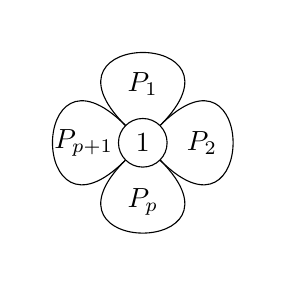
\begin{tikzpicture}
            \node[draw, circle] (1) at (0, 0) {$1$};
            \draw (1) to [in=135, out=45,  looseness=10] (1);
            \draw (1) to [in=45,  out=315, looseness=10] (1);
            \draw (1) to [in=225, out=315, looseness=10] (1);
            \draw (1) to [in=135, out=225, looseness=10] (1);

            \node at (0, 0.75)  {$P_1$};
            \node at (0.75, 0)  {$P_2$};
            \node at (0, -0.75) {$P_p$};
            \node at (-0.75, 0) {$P_{p+1}$};
        \end{tikzpicture}
    \end{center}

    Each of these is a cyclic group of order $p$. 

    Take $g \in G$, $P_i$ the cyclic group generated by $g$. \[
        g P_i g^{-1} = P_j
    \] for some cyclic group $P_j$.

    Let us call $\Phi(g) \in S_{p+1}$ such that \[
        g P_i g^{-1} = P_{\Phi(g)(i)}.
    \]

    In this way we have created a map \[
        \Phi: G \to S_{p+1}.
    \]

    We claim that $\Phi$ is a homomorphism.

    Pick $xy \in G$, $\begin{aligned}[t]
        (xy) P_i (xy)^{-1} &= x(y P_i y^{-1})x^{-1} \\
                           &= x P_{\Phi(y)(i)} x^{-1} \\
                           &= P_{\Phi(x)(\Phi(y)(i))}.
    \end{aligned}$

    Meanwhile, $(xy) P_i (xy)^{-1} = P_{\Phi(xy)(i)}$, so $\Phi(xy)(i) = \Phi(x)(\Phi(y)(i))$ for all $i$.

    Therefore, $\Phi(xy) = \Phi(x) \circ \Phi(y)$.

    {~~~}

    Thus, $\Phi: G \to S_{p+1}$ must satisfy \vspace{-1em} \[ 
        p^2 = | \ker{\Phi} | \cdot | \im{\Phi} |.
    \]

    If $\ker{\Phi} = \{ e \}$, then $| \im{\Phi} | = p^2$.

    This cannot happen, since $p^2$ is not a divisor of $(p+1)!$, the order of $S_{p+1}$.

    This is a violation of Lagrange's Theorem.

    Then, the kernel of $\Phi$ is not trivial.

    {~~~}

    There are elements $x \neq e$ such that \[
        x P_i x^{-1} = P_i \quad \text{for all } i.
    \]

    Suppose $P_i$ does not contain $x$, and consider $y$ a generator of $P_i$. 

    Then, $x y x^{-1} = y^n$ for some $n$. \[
        y^{2n} = (x y x^{-1}) (x y x^{-1}) = x y^2 x^{-1}
    \] 

    Continuing like this, \[
        x y^k x^{-1} = y^{kn}
    \]

    {~~~}

    The powers of $x$, $\{ 1, x, x^2, \dots, x^{p-1} \}$, move the elements of $P_i$ as follows:
    \begin{align*}
        x^2 y x^{-2} & = x (x y x^{-1}) x^{-1} \\
                     & = x y^n x^{-1}          \\
                     & = (x y x^{-1})^n        \\
                     & = (y^n)^n               \\
                     & = y^{n^2}.
    \end{align*}

    Continuing like this, \[
        x^k y x^{-k} = y^{n^k}.
    \]

    {~~~}

    Pick $k = p-1$, we know that $x^{p-1} = x^{-1}$, so \[
        x^{-1} y x = y^{n^{p-1}} = y
    \] by Fermat's Little Theorem.

    \begin{theorem}[Fermat's Little Theorem]\index{Fermat's Little Theorem}
        Let $p$ be a prime number, and $a$ be an integer not divisible by $p$. Then, \[
            a^{p-1} \equiv 1 \mod{p}.
        \]
    \end{theorem}

    This allows us to conclude the following face: \[
        \exists x, y \in G \text{ of order } p \text{ that commute}.
    \]

    Define \[
        \begin{matrix}[rccc]
            \Psi: & \Z/p\Z & \times  & \Z/p\Z \to G \\
                  & (m, n) & \mapsto & x^m y^n
        \end{matrix}
    \]

    \begin{claim}
        $\Phi$ is an isomorphism.
    \end{claim}

    \begin{listu}
        \item \textbf{Injectivity}
        
        $x^m y^n = 1 \implies x^m = y^{-n} \in P_i n P_j = \{ e \}$, where $x \in P_i$ and $y \in P_j$.

        \item \textbf{Surjectivity}
        
        Let $g \in G$. Then, $g = x^m y^n$ for some $m, n \in \Z/p\Z$.

        \item \textbf{Homomorphism}
        \vspace{-1em}
        \begin{align*}
            \Psi(m_1 + m_2, n_1 + n_2) & = x^{m_1 + m_2} y^{n_1 + n_2}     \\
                                       & = x^{m_1} x^{m_2} y^{n_1} y^{n_2} \\
                                       & = x^{m_1} y^{n_1} x^{m_2} y^{n_2} \\
                                       & = \Psi(m_1, n_1) \Psi(m_2, n_2)
        \end{align*}
    \end{listu}

    This completes the proof.
\end{proof}

\subsection{Hasse Diagram of Groups}

Consider the Hasse diagram of $D_6$. There are 2 elements that generate everything, $R$ and $S$. They satisfy $\begin{cases}
    R^6 = e \\
    S^2 = e \\
    SRS = R^5 
\end{cases}$

The elements are \begin{itemize}
    \item $e, R, R^2, R^3, R^4, R^5$
    \item $S, SR, SR^2, SR^3, SR^4, SR^5$
\end{itemize}

To build the Hasse diagram, we need the divisors of $| D_6 | = 12$. Hence, we have \[
    1, 2, 3, 4, 6, 12,
\] same as $C_{12}$. However, since $D_6$ is not cyclic, we do not know if the subgroups of $D_6$ are cyclic.

\subsubsection{Cyclic Subgroups of $D_6$}

% TODO

% See notes P.10. 

% On P.19, $\bar{S}$ means $S \langle R^2 \rangle$, similarly for all other elements with a bar.

\includepdf[pages=-,nup=2x3]{/Users/lance/Downloads/MAT301 S 2024 Lecture 10.pdf}